\documentclass{standalone}
\usepackage{tikz}
\usetikzlibrary{patterns, positioning}

\begin{document}
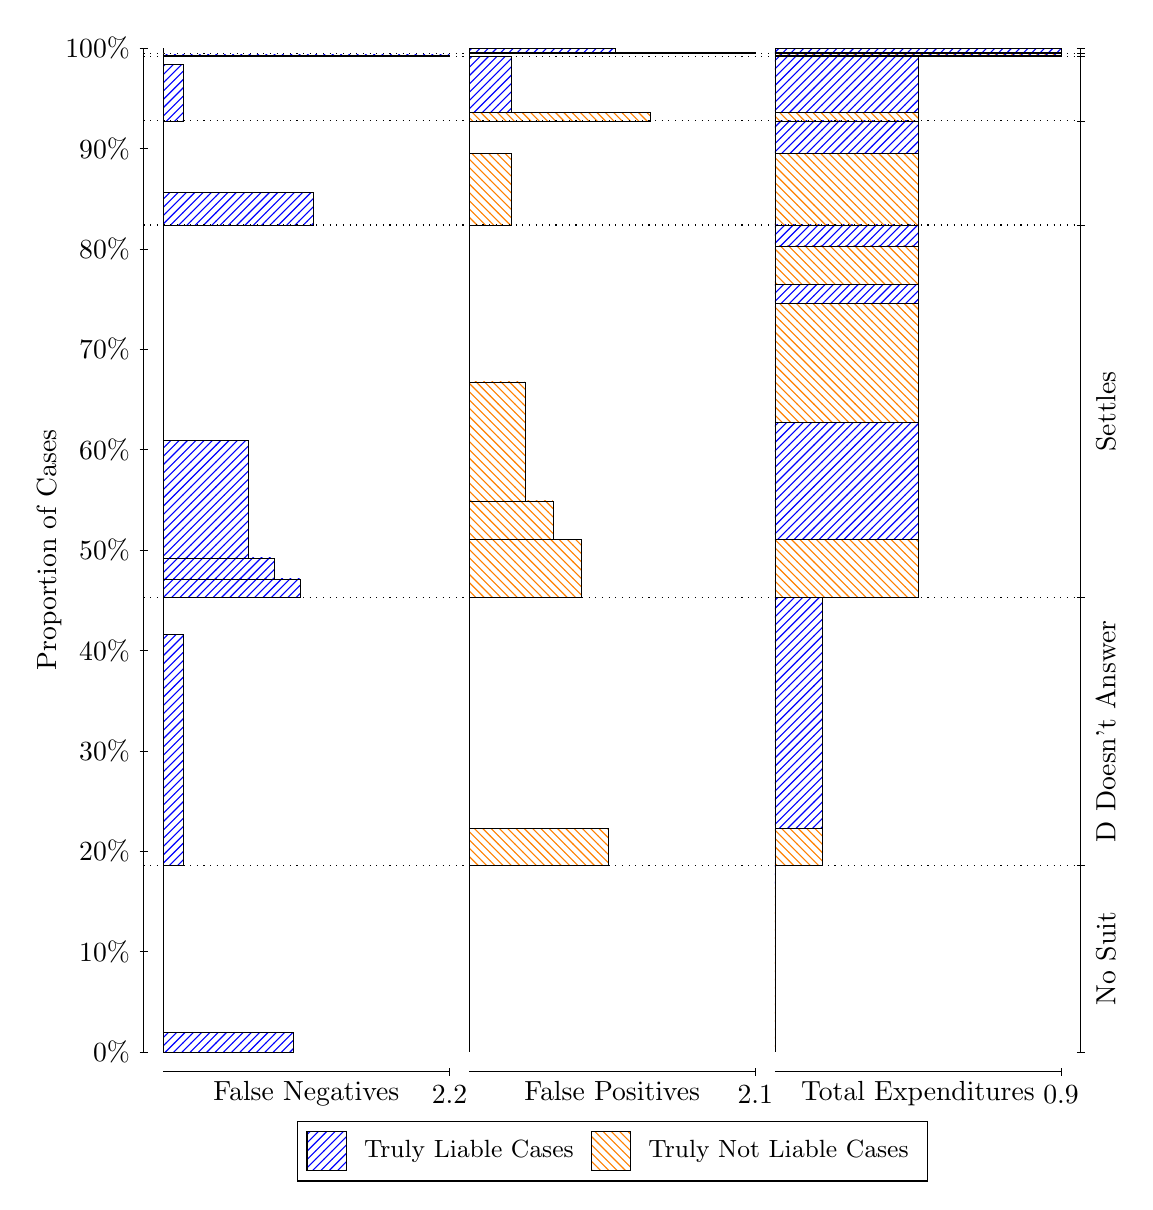
\begin{tikzpicture}
\draw[black, very thin] (1.5,1.75) -- (1.5,14.5);
\node[rotate=90, anchor=center] at (0.3, 8.125) {Proportion of Cases};
\draw[black, very thin] (1.45,1.75) -- (1.55,1.75);
\node[anchor=east] at (1.45, 1.75) {0\%};
\draw[black, very thin] (1.45,3.025) -- (1.55,3.025);
\node[anchor=east] at (1.45, 3.025) {10\%};
\draw[black, very thin] (1.45,4.3) -- (1.55,4.3);
\node[anchor=east] at (1.45, 4.3) {20\%};
\draw[black, very thin] (1.45,5.575) -- (1.55,5.575);
\node[anchor=east] at (1.45, 5.575) {30\%};
\draw[black, very thin] (1.45,6.85) -- (1.55,6.85);
\node[anchor=east] at (1.45, 6.85) {40\%};
\draw[black, very thin] (1.45,8.125) -- (1.55,8.125);
\node[anchor=east] at (1.45, 8.125) {50\%};
\draw[black, very thin] (1.45,9.4) -- (1.55,9.4);
\node[anchor=east] at (1.45, 9.4) {60\%};
\draw[black, very thin] (1.45,10.675) -- (1.55,10.675);
\node[anchor=east] at (1.45, 10.675) {70\%};
\draw[black, very thin] (1.45,11.95) -- (1.55,11.95);
\node[anchor=east] at (1.45, 11.95) {80\%};
\draw[black, very thin] (1.45,13.225) -- (1.55,13.225);
\node[anchor=east] at (1.45, 13.225) {90\%};
\draw[black, very thin] (1.45,14.5) -- (1.55,14.5);
\node[anchor=east] at (1.45, 14.5) {100\%};

\draw[black, very thin] (13.4,1.75) -- (13.4,14.5);
\draw[black, very thin] (13.35,1.75) -- (13.45,1.75);
\node[anchor=west] at (13.35, 1.75) {};
\draw[black, very thin] (13.35,4.1224) -- (13.45,4.1224);
\node[anchor=west] at (13.35, 4.1224) {};
\draw[black, very thin] (13.35,7.519) -- (13.45,7.519);
\node[anchor=west] at (13.35, 7.519) {};
\draw[black, very thin] (13.35,12.253) -- (13.45,12.253);
\node[anchor=west] at (13.35, 12.253) {};
\draw[black, very thin] (13.35,13.576) -- (13.45,13.576);
\node[anchor=west] at (13.35, 13.576) {};
\draw[black, very thin] (13.35,14.396) -- (13.45,14.396);
\node[anchor=west] at (13.35, 14.396) {};
\draw[black, very thin] (13.35,14.431) -- (13.45,14.431);
\node[anchor=west] at (13.35, 14.431) {};
\draw[black, very thin] (13.35,14.5) -- (13.45,14.5);
\node[anchor=west] at (13.35, 14.5) {};

\draw[black, very thin, pattern color=blue, pattern=north east lines] (1.75,1.75) rectangle (3.4015,1.9996);
\draw[black, very thin, pattern color=orange, pattern=north west lines] (1.75,1.9996) rectangle (1.75,4.1224);
\draw[black, very thin, pattern color=blue, pattern=north east lines] (1.75,4.1224) rectangle (1.9977,7.0546);
\draw[black, very thin, pattern color=orange, pattern=north west lines] (1.75,7.0546) rectangle (1.75,7.519);
\draw[black, very thin, pattern color=blue, pattern=north east lines] (1.75,7.519) rectangle (3.4841,7.7578);
\draw[black, very thin, pattern color=blue, pattern=north east lines] (1.75,7.7578) rectangle (3.1538,8.0249);
\draw[black, very thin, pattern color=blue, pattern=north east lines] (1.75,8.0249) rectangle (2.8235,9.5125);
\draw[black, very thin, pattern color=orange, pattern=north west lines] (1.75,9.5125) rectangle (1.75,12.253);
\draw[black, very thin, pattern color=blue, pattern=north east lines] (1.75,12.253) rectangle (3.6492,12.67);
\draw[black, very thin, pattern color=orange, pattern=north west lines] (1.75,12.67) rectangle (1.75,13.576);
\draw[black, very thin, pattern color=blue, pattern=north east lines] (1.75,13.576) rectangle (1.9977,14.29);
\draw[black, very thin, pattern color=orange, pattern=north west lines] (1.75,14.29) rectangle (1.75,14.396);
\draw[black, very thin, pattern color=blue, pattern=north east lines] (1.75,14.396) rectangle (5.3833,14.413);
\draw[black, very thin, pattern color=orange, pattern=north west lines] (1.75,14.413) rectangle (1.75,14.431);
\draw[black, very thin, pattern color=orange, pattern=north west lines] (1.75,14.431) rectangle (1.75,14.449);
\draw[black, very thin, pattern color=blue, pattern=north east lines] (1.75,14.449) rectangle (1.75,14.5);
\draw[black, very thin, pattern color=orange, pattern=north west lines] (5.6333,1.75) rectangle (5.6333,3.8728);
\draw[black, very thin, pattern color=blue, pattern=north east lines] (5.6333,3.8728) rectangle (5.6333,4.1224);
\draw[black, very thin, pattern color=orange, pattern=north west lines] (5.6333,4.1224) rectangle (7.4057,4.5867);
\draw[black, very thin, pattern color=blue, pattern=north east lines] (5.6333,4.5867) rectangle (5.6333,7.519);
\draw[black, very thin, pattern color=orange, pattern=north west lines] (5.6333,7.519) rectangle (7.0512,8.26);
\draw[black, very thin, pattern color=orange, pattern=north west lines] (5.6333,8.26) rectangle (6.6967,8.7498);
\draw[black, very thin, pattern color=orange, pattern=north west lines] (5.6333,8.7498) rectangle (6.3423,10.259);
\draw[black, very thin, pattern color=blue, pattern=north east lines] (5.6333,10.259) rectangle (5.6333,12.253);
\draw[black, very thin, pattern color=orange, pattern=north west lines] (5.6333,12.253) rectangle (6.165,13.159);
\draw[black, very thin, pattern color=blue, pattern=north east lines] (5.6333,13.159) rectangle (5.6333,13.576);
\draw[black, very thin, pattern color=orange, pattern=north west lines] (5.6333,13.576) rectangle (7.9374,13.682);
\draw[black, very thin, pattern color=blue, pattern=north east lines] (5.6333,13.682) rectangle (6.165,14.396);
\draw[black, very thin, pattern color=orange, pattern=north west lines] (5.6333,14.396) rectangle (5.6333,14.414);
\draw[black, very thin, pattern color=blue, pattern=north east lines] (5.6333,14.414) rectangle (5.6333,14.431);
\draw[black, very thin, pattern color=orange, pattern=north west lines] (5.6333,14.431) rectangle (9.2667,14.449);
\draw[black, very thin, pattern color=blue, pattern=north east lines] (5.6333,14.449) rectangle (7.4943,14.5);
\draw[black, very thin, pattern color=orange, pattern=north west lines] (9.5167,1.75) rectangle (9.5167,3.8728);
\draw[black, very thin, pattern color=blue, pattern=north east lines] (9.5167,3.8728) rectangle (9.5167,4.1224);
\draw[black, very thin, pattern color=orange, pattern=north west lines] (9.5167,4.1224) rectangle (10.122,4.5867);
\draw[black, very thin, pattern color=blue, pattern=north east lines] (9.5167,4.5867) rectangle (10.122,7.519);
\draw[black, very thin, pattern color=orange, pattern=north west lines] (9.5167,7.519) rectangle (11.333,8.26);
\draw[black, very thin, pattern color=blue, pattern=north east lines] (9.5167,8.26) rectangle (11.333,9.7476);
\draw[black, very thin, pattern color=orange, pattern=north west lines] (9.5167,9.7476) rectangle (11.333,11.257);
\draw[black, very thin, pattern color=blue, pattern=north east lines] (9.5167,11.257) rectangle (11.333,11.496);
\draw[black, very thin, pattern color=orange, pattern=north west lines] (9.5167,11.496) rectangle (11.333,11.986);
\draw[black, very thin, pattern color=blue, pattern=north east lines] (9.5167,11.986) rectangle (11.333,12.253);
\draw[black, very thin, pattern color=orange, pattern=north west lines] (9.5167,12.253) rectangle (11.333,13.159);
\draw[black, very thin, pattern color=blue, pattern=north east lines] (9.5167,13.159) rectangle (11.333,13.576);
\draw[black, very thin, pattern color=orange, pattern=north west lines] (9.5167,13.576) rectangle (11.333,13.682);
\draw[black, very thin, pattern color=blue, pattern=north east lines] (9.5167,13.682) rectangle (11.333,14.396);
\draw[black, very thin, pattern color=orange, pattern=north west lines] (9.5167,14.396) rectangle (13.15,14.414);
\draw[black, very thin, pattern color=blue, pattern=north east lines] (9.5167,14.414) rectangle (13.15,14.431);
\draw[black, very thin, pattern color=orange, pattern=north west lines] (9.5167,14.431) rectangle (13.15,14.449);
\draw[black, very thin, pattern color=blue, pattern=north east lines] (9.5167,14.449) rectangle (13.15,14.5);
\draw[black, dotted] (1.5,4.1224) -- (13.4,4.1224);
\draw[black, dotted] (1.5,7.519) -- (13.4,7.519);
\draw[black, dotted] (1.5,12.253) -- (13.4,12.253);
\draw[black, dotted] (1.5,13.576) -- (13.4,13.576);
\draw[black, dotted] (1.5,14.396) -- (13.4,14.396);
\draw[black, dotted] (1.5,14.431) -- (13.4,14.431);
\draw[black, very thin] (1.75,1.5) -- (5.3833,1.5);
\node[anchor=north] at (3.5667, 1.5) {False Negatives};
\draw[black, very thin] (5.3833,1.45) -- (5.3833,1.55);
\node[anchor=north] at (5.3833, 1.45) {2.2};

\draw[black, very thin] (5.6333,1.5) -- (9.2667,1.5);
\node[anchor=north] at (7.45, 1.5) {False Positives};
\draw[black, very thin] (9.2667,1.45) -- (9.2667,1.55);
\node[anchor=north] at (9.2667, 1.45) {2.1};

\draw[black, very thin] (9.5167,1.5) -- (13.15,1.5);
\node[anchor=north] at (11.333, 1.5) {Total Expenditures};
\draw[black, very thin] (13.15,1.45) -- (13.15,1.55);
\node[anchor=north] at (13.15, 1.45) {0.9};

\node[black, centered, rotate=90] at (13.72, 2.9362) {No Suit};
\node[black, centered, rotate=90] at (13.72, 5.8207) {D Doesn't Answer};
\node[black, centered, rotate=90] at (13.72, 9.8859) {Settles};





\draw (7.449999999999999,1.5) node[draw=none] (baseCoordinate) {};
\begin{scope}[align=center]
        \matrix[scale=0.5, draw=black, below=0.5cm of baseCoordinate, nodes={draw}, column sep=0.1cm]{
            \node[rectangle, draw, minimum width=0.5cm, minimum height=0.5cm, pattern=north east lines, pattern color=blue] {}; &
            \node[draw=none, font=\small] (B) {Truly Liable Cases}; &
            \node[rectangle, draw, minimum width=0.5cm, minimum height=0.5cm, pattern=north west lines, pattern color=orange] {}; &
            \node[draw=none, font=\small] (B) {Truly Not Liable Cases}; \\
            };
\end{scope}

\end{tikzpicture}
\end{document}